Wolfenstein 3D was released in May 1992 and shortly after achieved legendary status. The impact was such that it is credited for creating the First Person Shooter genre. Universally acclaimed, the beautiful graphics, crisp digitalized sounds, engaging musics and outstanding game design made the game engine sing. Within a year more than 100,000 units had been sold, bringing fame and a little bit of fortune to the team of people who built it: id Software.\\
\\
The many fans did not stop at beating the game. Because they wanted to modify it, they started to explore and reverse engineered parts of it. Within a few months the assets formats were well known and people released mods\footnote{MODified version.} with altered graphics, sounds effects, music and maps. The core of the game however, the 3D engine and the secrets of its speed remained mostly unknown.\\
\\
It was kept secret for an obvious reason:. A good game engine was considered the main asset of a game company. As a mean to outperform competitors it was a good business practice to keep other programmers  uneducated in order to gain technological advantage and generate profit.\\
\\
But a few people within id Software did not see things that way. Instead of going along with business common sense, they wanted to embrace players enthusiasm and fully open the source code to the public. After many internal debate, id Software did the unthinkable: On July 21, 1995 they uploaded a zip archive on \emph{ftp.idsoftware.com} containing the full source code of the engine with all instructions to build it.\\

 \begin{fancyquotes}
   Programming is not a zero-sum game. Teaching something to a fellow programmer doesn't take it away from you. I'm happy to share what I can, because I'm in it for the love of programming.\\
   \\
\textbf{John Carmack - Programmer}
 \end{fancyquotes}\\
\\
Pessimists would have forecasted the demise of a company foolish enough to give away its technology: Nobody had ever released the source of a mondial hit. But instead of destroying them, it turned id Software into icon. A monument dedicated to the Right Thing\footnote{"Hackers: Heroes of the Computer Revolution" by Steven Levy.} that gamers and programmers could relate to.\\
\\
Sharing their knowledge enabled innumerable programers to become better engineers. It also allowed the software to live long after the target hardware and operating system died. With access to the source, programmers were able to port the engine to new hardware and operating systems: Twenty years after the release of Wolfenstein 3D you can still play the game on anything with a CPU, RAM and a framebuffer. \\
\\
A second unexpected side effect of opening the source was the creation of a window back in time looking right into 1992. As a technical writer on \emph{fabiensanglard.net} I thought i would never take a look at this old thing. But when out of curiosity I took a peek, I could not stop reading: I was mesmerized. The more I read, the more I came to realize one very important thing: The IBM PC was designed for office work, not gaming. It was meant to crunch integers and display static images.\\
\\ 
Part of the beauty of Wolfenstein 3D engine is that its repurpose the hardware to perform something it was not meant created to do.\\
\\
It would be an easy mistake to look at a CPU mips\footnote{Million Instructions Per Second.} graph such as Figure \ref{fig:game_console_vs_PC} comparing the power of a PC with the gaming systems of the time only to conclude that because PC were so powerful it was ''easy'' to write a game for this machine. \\
\\
\begin{figure}[H]
\centering
  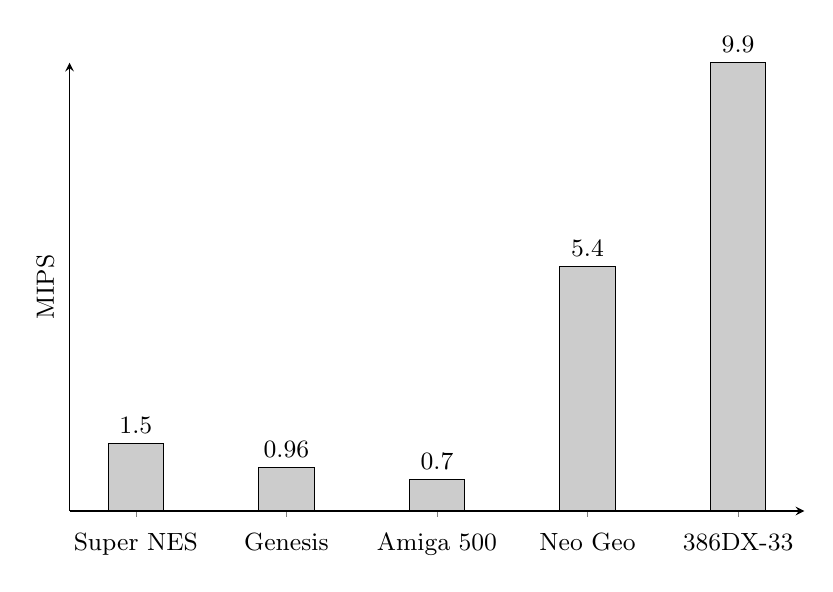
\begin{tikzpicture}[font=\small]
    \begin{axis}[
      width=0.9\textwidth,
      height=0.6\textwidth,
      ybar=6pt,
      bar width=20pt,
      ylabel={MIPS},
      ymin=0,
      ytick=\empty,
      xtick=data,
      axis x line=bottom,
      axis y line=left,
      enlarge x limits=0.11,
      symbolic x coords={Super NES,Genesis,Amiga 500,Neo Geo,386DX-33},
      xticklabel style={anchor=base,yshift=-\baselineskip},
      nodes near coords={\pgfmathprintnumber\pgfplotspointmeta}
    ]
      \addplot[fill=black!20,draw=black] coordinates {
        (Super NES,1.5)
        (Genesis,0.96)
        (Amiga 500,0.7)
        (Neo Geo,5.4)
        (386DX-33,9.9)
      };
    \end{axis}
   \end{tikzpicture}
   \caption{Game Console Vs PC.} \label{fig:game_console_vs_PC}
 \end{figure}
 
That would be omitting the fact that game console were designed around animation. They all featured coprocessors and Graphic Processing Unit relying on tile engines. Animating a sprite on the screen was just about to update its $(x,y)$ coordinates.\\
\\
On the contrary, smooth animation on a PC was next to impossible. Not to mention many other obstacles related to the CPU, complicated RAM, distorted screen and operating system awful limitations. I saw beauty in this ability to repurpose the machine. It takes optimist, creativity, passion, craziness and dedication to do that.\\
\\
This book is broken down in three parts and details:\\
\begin{itemize}
\item Hardware: The limitations of the machine.
\item People: The team and workflow they followed to produce the software
\item Software: The engine pushing the hardware as far as it can.
\end{itemize}

 \textbf{\underline{Disclaimer :}} The description that follows is technical and will most likely appeal to programmers. If you are more into the human aspect of game programming I would recommend instead to read David Kushner's chef d'oeuvre: "Masters of Doom: How Two Guys Created an Empire and Transformed Pop Culture".